%% ------------------------------------------------------------------------- %%
\chapter{Programação Dinâmica}
\label{cap:programacao-dinamica}

\section{Introdução}

Neste capítulo apresentaremos o primeiro algoritmo realmente eficiente para calcular o \LCA\ entre dois vértices em uma árvore enraizada utilizando programação dinâmica. Este algoritmo terá complexidade de tempo $O(log(n))$ por consulta, onde $log(n)$ é o logaritmo na base 2 de $n$ - a quantidade de vértices na árvore.

\section{Descrição}

A ideia deste algoritmo segue a mesma dos capítulos anteriores: primeiro são pré-calculados ancestrais dos vértices para depois realizar as consultas.

Para cada vértice serão pré-computados os ancestrais cuja profundidade na árvore é menor do que a sua em uma potência de dois - ou seja - 1, 2, 4, 8, ... , $h$ níveis acima dele, onde $h$ é a maior potência de dois que não ultrapasse a altura da árvore. Em outras palavras, para cada vértice serão pré-calculados até $log(n)$ ancestrais diferentes.

Para ilustrar este pré-processamento, introduzimos a figura a seguir:

\begin{figure}[htb]
\begin{center}
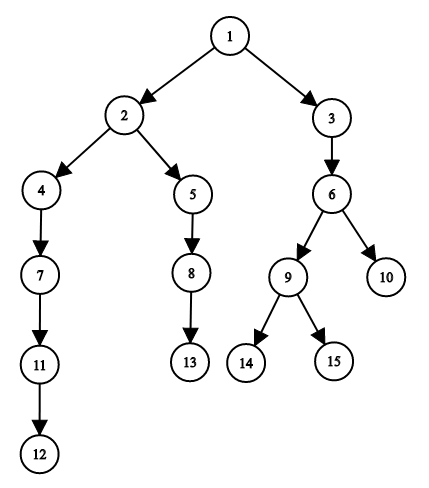
\includegraphics[width=7.2cm]{images/graph_dp.png}
\end{center}
\caption{\label{fig:arvore-6}Árvore enraizada de altura 6.}
\end{figure}

Após o pré-processamento, teríamos como os ancestrais, para os vértices 12 e 15:

\begin{itemize}
    \item Vértice 11

    \begin{table}[htb]
    \centering
    \begin{tabular}{|l|c|c|c|c|c|c|c|c|c|c|c|c|c|c|}
    \hline
    Altura relativa & -1 & -2 & -4 \\ \hline
    Ancestral       & 7 & 4  & 1 \\ \hline
    \end{tabular}
    \caption{Ancestrais relativos do vértice 12}
    \end{table}
    
    \item Vértice 15
    
    \begin{table}[htb]
    \centering
    \begin{tabular}{|l|c|c|c|c|c|c|c|c|c|c|c|c|c|c|}
    \hline
    Altura relativa & -1 & -2 & -4 \\ \hline
    Ancestral       & 9  & 6  & 1 \\ \hline
    \end{tabular}
    \caption{Ancestrais relativos do vértice 15}
    \end{table}

\end{itemize}

Por conveniência, a partir de agora vamos nos referir à cada ancestral de um vértice $v$ como $ancestral_v(2^i)$ para todo inteiro $i$.

Agora, para calcular o \LCA\ entre dois vértices $a$ e $b$ faremos o que já vimos em todos os capítulos anteriores: vamos caminhar até a raiz com ambos. A maneira que faremos isso desta vez é dando pulos de tamanho "potência de dois"\  com auxílio dos valores que já foram pré-computados. Além disso, cada pulo é de um tamanho diferente.

Vamos assumir sem perda de generalidade que $b$ é mais profundo do que $a$. Inicialmente, são feitos sucessivos pulos suficientes para que $a$ e $b$ estejam exatamente no mesmo nível. Por exemplo, se a profundidade de $a$ é 3 e a de $b$ é 6, devemos subir $b$ em $6 - 3 = 3$ níveis: o que equivale a um pulo de tamanho 2 e um pulo de tamanho 1. Provaremos adiante que sempre conseguimos igualar os níveis dos vértices dando pulos diferentes de tamanho de alguma potência de dois cada.

Tendo $a$ e $b$ agora no mesmo nível, podemos checar se eles são iguais. Se forem, isso signfica que $a$ estava originalmente no caminho de $b$ até a raiz e que portanto ela é o \LCA. Caso contrário, devemos encontrar o maior tamanho de um pulo para subir simultaneamente os vértices $a$ e $b$ de forma que ainda sejam diferentes. Encontraremos este valor dando pulos distintos de tamanho de alguma potência de dois. A figura a seguir um possível cenário:

\begin{figure}[htb]
\begin{center}
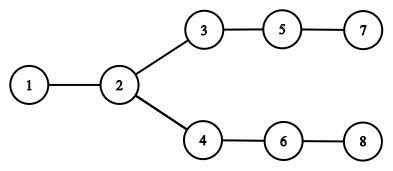
\includegraphics{images/graph_dp2.png}
\end{center}
\caption{\label{fig:arvore-5}Árvore enraizada de altura 5.}
\end{figure}


Consideremos $a = 7$ e $b = 8$. Vamos listar os possíveis valores a serem escolhidos para subir simultaneamente $a$ e $b$. Note que ao subir $2^3 = 8$ ou mais níveis a restrição da altura máxima da árvore seria violada, e por isso a última potência de dois a ser considerada é $2^2 = 4$.

\begin{itemize}
    \item \textbf{4}: Ao subir 4 níveis, $a$ e $b$ são iguais (ambos = $1$). Não o fazemos.
    \item \textbf{2}: Ao subir 2 níveis, $a$ e $b$ são diferentes. Então atualizamos $a$ e $b$ para tais ancestrais. Agora $a = 3$ e $b = 4$
    \item \textbf{1}: Ao subir 1 nível, os valores atualizados de $a$ e $b$ são iguais (ambos = $2$). Não o fazemos.
\end{itemize}

Em outras palavras, o que encontramos são os dois vértices distintos mais próximos à raiz que contém, respectivamente, os vértices $a$ e $b$ em suas sub-árvores. Assim, o pai destes vértices será o \LCA\, já que será o primeiro vértice que contém ambos $a$ e $b$ em sua sub-árvore.

\vspace{1cm}

Voltando à figura \ref{fig:arvore-6}, vamos simular os passos completos para encontrar o \LCA(12, 15):

\begin{itemize}
    \item Vértices 12 e 15 não estão na mesma altura. O vértice 12 é mais profundo, então vamos subi-lo em direção à raiz.
    \item A diferença das profundidades de 12 e 15 é de um. Então agora seu novo valor é $ancestral_{12}(1) =$ vértice 11.
    \item Agora, vamos determinar qual é o o maior inteiro $i$ tal que $ancestral_{11}(i) \neq ancestral_{15}(i)$. Testando as potências de dois, da maior para a menor, tentaremos primeiro subir 4 níveis - o que resultaria em ambos irem até o vértice $1$. Então, testamos 2 níveis - o que resulta nos vértices $4$ e $6$, respectivamente. Como são distintos, vamos para eles. Finalmente, tentamos subir 1 nível - o que resulta nos vértices $2$ e $3$ - ainda distintos. Vamos para eles.
    \item Finalmente, sabemos que os últimos dois vértices antes do \LCA\ são $2$ e $3$, então basta retornar o pai de qualquer um deles para obter o \LCA: o vértice $1$.
\end{itemize}


\vspace{10cm}

\section{Algoritmo}

Vamos dividir nosso algoritmo em duas partes: pré-processamento da matriz de programação dinâmica e a função de obtenção do \LCA\ entre dois vértices $a$ e $b$.

\begin{algorithm}[H]
\caption{Cálculo da matriz de programação dinâmica ($pd$)}
\begin{algorithmic}[1]
\Function{\textsc{CalculaPD}}{}
    \For{cada $nivel$ em $logNiveis$}
        \For{cada $vertice$ em $vertices$}
            \If{$nivel = 0$}
                \State $pd[vertice][nivel] \rec pai[vertice]$
            \Else
                \State $pd[vertice][nivel] \rec pd[pd[vertice[nivel-1]][nivel-1]$
            \EndIf
        \EndFor
    \EndFor
\EndFunction
\end{algorithmic}
\end{algorithm}


\begin{algorithm}[H]
\caption{Obtenção do \LCA}
\begin{algorithmic}[1]
\Function{\textsc{CalculaPD}}{a,\ b}
    \If{$profundidade[b] < profundidade[a]$}
        \State $troca(a, b)$
    \EndIf
    \State $bAtual \rec b$
    \For {$i \rec logNiveis;\ i \geq 0;\ i\ -= 1$}
        \If{$profundidade[bAtual] - 2^i \geq profundidade[a]$}
            \State $bAtual \rec pd[b][i]$
        \EndIf
    \EndFor
    \State $b \rec bAtual$
    \If{$a = b$}
        \\\hspace{11mm} \Return $a$
    \EndIf
    \For{$i \rec logNiveis;\ i \geq 0;\ i\ -= 1$}
        \If{$pd[a][i] \neq pd[b][i]$}
            \State $a \rec pd[a][i]$
            \State $b \rec pd[b][i]$
        \EndIf
    \EndFor
    \\\hspace{5mm} \Return $pai[a]$
\EndFunction
\end{algorithmic}
\end{algorithm}

\section{Corretude}

TODO

\section{Complexidade}

TODO
